\documentclass[12pt,oneside,a4paper]{article}

\usepackage[backend=biber,style=numeric]{biblatex}
\usepackage{xcolor}
\usepackage{todonotes}
\usepackage{amsmath}
\usepackage{multicol}
\usepackage{caption}
\usepackage{hyperref}
\usepackage{graphicx}
\usepackage{listings}
\lstset{
	frame=top,frame=bottom,
	language=C,
	basicstyle=\small\normalfont,
	xleftmargin=\parindent,
	keywordstyle=\color{green!40!black},
	%  commentstyle=\itshape\color{purple!40!black},
	%  identifierstyle=\color{blue},
	%  stringstyle=\color{orange},
	morekeywords={in, globaldata, procedure, input, output, behavior, end, XOR, NOT, AND}, % keyword to highlight
	%  captionpos=t,
	tabsize=2,
	numbers=left,
	stepnumber=1,                   % the step between two line-numbers.        
	numbersep=5pt,
	framexleftmargin=10pt,
	title=\lstname,
	captionpos=t,
	showspaces=false,
}
\DeclareCaptionFormat{listing}{\rule{\dimexpr\textwidth\relax}{0.4pt}\par\vskip1pt#1#2#3}
\captionsetup[lstlisting]{format=listing,singlelinecheck=false, margin=0pt,labelsep=space,labelfont=bf}

\usepackage{booktabs}
\usepackage[noabbrev,capitalise]{cleveref}
\crefname{listing}{algorithm}{algorithms}
\Crefname{listing}{Algorithm}{Algorithms}
\renewcommand\lstlistingname{Algorithm}
\def\lstlistingcrefname{Algorithm}
\usepackage{url}

\addbibresource{biblio.bib}

\title{\textbf{Parallel Kmenas Images Compressor}}

\author{Leonardo Ignazio Pagliochini \\ Francesco Rosnati}

\date{\today}

\begin{document}


\begin{titlepage}
	\centering
	\clearpage
	\maketitle
	\thispagestyle{empty}
	\vspace*{3cm}
	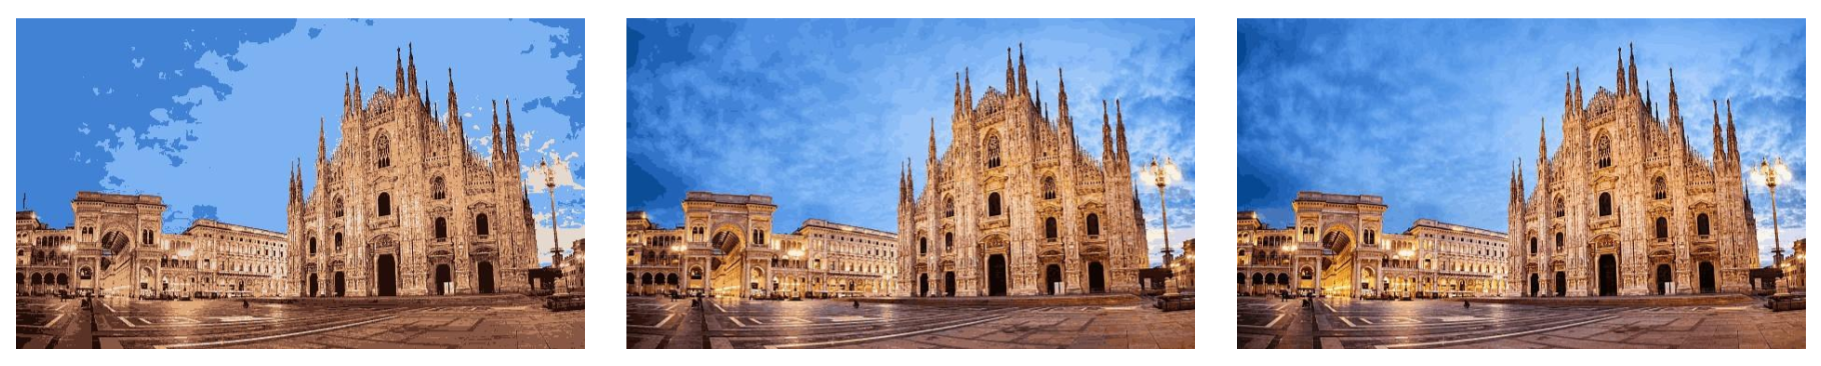
\includegraphics[width=14cm]{milanoCompressed.png} % qui mettete il vostro logo, o cancellate la linea
	\vfill
	\centering
	
\includegraphics{logo_polimi.png}
\end{titlepage}


\begin{abstract}
In this report, we present a parallel implementation of the K-means algorithm for image compression. 
The algorithm is implemented in C++ using OpenMP, MPI and CUDA to parallelize the computation. 
The report describes the algorithm, the implementation, and the results of the experiments. 
The results show that the parallel implementations are faster than the sequential one, and that the CUDA implementation is the 
fastest among the three parallel versions. The report also discusses the limitations of the parallel implementation and possible future improvements.
\end{abstract}

\section{Introduction} \label{sec:intro}
K-means is a widely used technique in data analysis and machine learning for grouping similar data points together. It is based on the heuristic that data points that are close to each other in the feature space are likely to belong to the same group. The algorithm works by 
iteratively assigning data points to the nearest cluster center and then updating the cluster centers based on the new assignments. The algorithm converges when the cluster centers no longer change significantly between iterations.
Differently from other clasterin algorithms, K-means needs to know the number of clusters in advance. This is a limitation of the algorithm, but it is also one of its strengths, as it allows the user to specify the number of clusters based on domain knowledge or other criteria.
In particular in this project we are interested in the application of the K-means algorithm to image compression to reduce the number of colors in an image. The idea is to represent the image with a smaller number of colors, while preserving the overall structure of the image. 
This can be useful for reducing the size of the image file, for example to speed up the loading of web pages or to save storage space.

\section{The Kmeans Algorithm} \label{sec:sec1}
In this section we describe the K-means algorithm in detail. To understand the algorithm, we first need to define some terms.\\
Let $X = \{x_1, x_2, \ldots, x_n\}$ be a set of data points in a $d$-dimensional space, where $x_i \in \mathbb{R}^d$.\\
The goal of the K-means algorithm is to partition the data points into $k$ clusters, where $k$ is a user-specified parameter.
The algorithm works as follows:
\begin{enumerate}
	\item Initialize the cluster centers $\mu_1, \mu_2, \ldots, \mu_k$ randomly or using some other heuristic.
	\item Assign each data point $x_i$ to the nearest cluster center $\mu_j$.
	\item Update the cluster centers $\mu_j$ by taking the mean of all data points assigned to cluster $j$.
	\item Repeat steps 2 and 3 until the cluster centers no longer change significantly between iterations.
\end{enumerate}
Here we present the pseudocode of the K-means algorithm.
\begin{lstlisting}[label={list:kmeans},caption={K-means algorithm}]
	def Kmeans(X, k):
	# Initialize the cluster centers
	for i in range(k):
		mu_i = random_point()
	
	# Main loop
	while True:
		# Assign data points to clusters
		for i in range(n):
			j = argmin_j ||x_i - mu_j||
			C_j = C_j + {x_i}
		
		# Update cluster centers
		for j in range(k):
			mu_j = (1/|C_j|) * sum(x for x in C_j)
		
		# Check for convergence
		if sum(||mu_j - mu_j_old|| for j in range(k)) < epsilon:
			break
\end{lstlisting}
Where:
\begin{itemize}
	\item $X$ is the set of data points
	\item $k$ is the number of clusters
	\item $n$ is the number of data points
	\item $\mu_i$ is the cluster center for cluster $i$
	\item $C_j$ is the set of data points assigned to cluster $j$
	\item $||x_i - mu_j||$ is the Euclidean distance between data point $x_i$ and cluster center $\mu_j$
	\item $argmin_j ||x_i - mu_j||$ is the index of the cluster center closest to data point $x_i$
	\item $epsilon$ is a small positive number that determines the convergence threshold
\end{itemize}



\subsection{The Image Compression} \label{sec:sub1}





\printbibliography

\end{document}


